\section{Dwi Yulianingsih}
\subsection{Teori}
\subsubsection{soal 1}
Matplotlib adalah librari plotting 2D Python yang menghasilkan gambar  publikasi bermutu di dalam berbagai format hardcopy dan lingkungan interaktif sepanjang platform. matplotlib dapat digunakan di dalam script Python, shell Python dan ipython), server aplikasi web, dan enam GUI toolkit. matplotlib mencoba untuk membuat hal mudah menjadi lebih mudah dan hal sulit menjadi mungkin. Kamu dapat membuat plot, histogram, power spectra, grafik batang, grafik error, scatterplot, dll, hanya dengan beberapa baris code.

\subsubsection{soal 2}
Pada Matplotlib untuk membuat sumbu X dan Y dapat dilakukan dengan cara yaitu :
\lstinputlisting[firstline=12, lastline=13]{src/6/1174009/chapter6.py}

\subsubsection{soal 3}
\begin{itemize}
\item Sebuah plot sebaran/titik adalah sebuah grafik yang menunjukkan hubungan antara dua set data.
\lstinputlisting[firstline=20, lastline=24]{src/6/1174009/chapter6.py}
\begin{figure}[H]
\centering
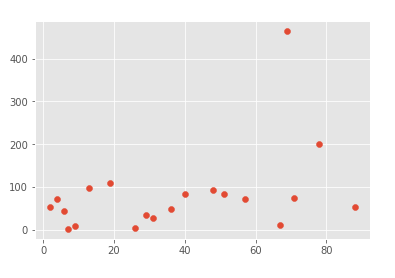
\includegraphics[width=7cm]{figures/6/1174009/1b.png}
\caption{Plot sebaran}
\label{dwiyul}
\end{figure}

\item Sebuah histogram adalah grafik yang menampilkan frekuensi data menggunakan batang, dimana angka dikelompokkan dalam rentang tertentu. Dengan kata lain, frekuensi setiap elemen data di dalam daftar ditunjukkan menggunakan histogram. Angka yang dikelompokkan dalam bentuk rentang tertentu disebut bins.
\lstinputlisting[firstline=27, lastline=31]{src/6/1174009/chapter6.py}
\begin{figure}[H]
\centering
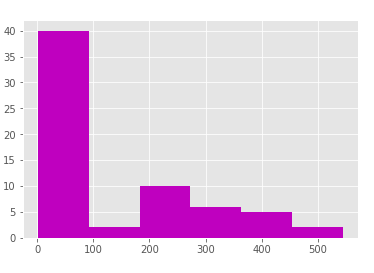
\includegraphics[width=7cm]{figures/6/1174009/1c.png}
\caption{Histogram}
\label{dwiyul}
\end{figure}

\item Menggambar sebuah plot garis menggunakan matplotlib. Dalam kasus ini, kita akan menggunakan matplotlib.pyplot, yang menyediakan sebuah framework plotting seperti MATLAB. Dengan kata lain, itu menyediakan sebuah koleksi function bergaya command yang membuat matplotlib berkerja seperti MATLAB.
\lstinputlisting[firstline=12, lastline=17]{src/6/1174009/chapter6.py}
\begin{figure}[H]
\centering
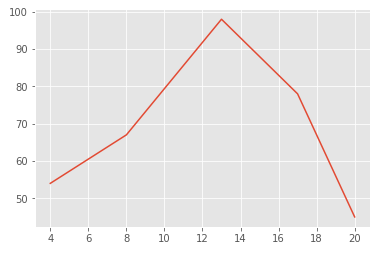
\includegraphics[width=7cm]{figures/6/1174009/1a.png}
\caption{plot garis}
\label{dwiyul}
\end{figure}

\item pie chart adalah diagram yang digunakan untuk membandingkan antar bagian terhadap total. biasanya pie chart dalam bentuk persentase karena nilainya merupakan bagian-bagian yang dijumlah menjadi satu. sehingga bisa lihat kontribusi paling besar atau paling kecil dalam membentuk nilai. Pie chart digunakan untuk perbandingan yang sedikit. pie chart digunakan untuk membandingkan antar bagian terhadap total.
\lstinputlisting[firstline=34, lastline=55]{src/6/1174009/chapter6.py}
\begin{figure}[H]
\centering
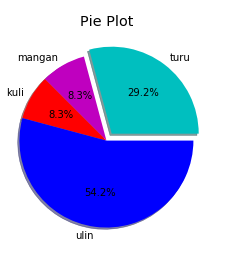
\includegraphics[width=7cm]{figures/6/1174009/1d.png}
\caption{pie chart}
\label{dwiyul}
\end{figure}

\item Bagan area benar-benar mirip dengan bagan garis, kecuali area antara sumbu x dan garis diisi dengan warna atau bayangan. Ini mewakili evolusi variabel numerik mengikuti variabel numerik lainnya. Jika kamu ingin mewakili evolusi ini untuk beberapa grup dalam waktu yang bersamaan, Anda mungkin tertarik dengan bagan area bertumpuk, di mana setiap grup ditampilkan satu sama lain.
\lstinputlisting[firstline=58, lastline=77]{src/6/1174009/chapter6.py}
\begin{figure}[H]
\centering
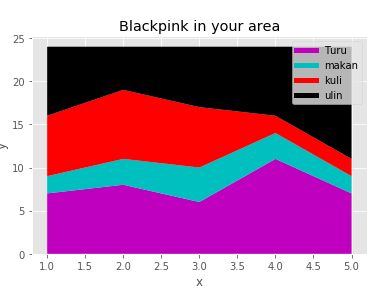
\includegraphics[width=7cm]{figures/6/1174009/1e.png}
\caption{bagan area}
\label{dwiyul}
\end{figure}

\end{itemize}

\subsubsection{soal 4}
Legenda adalah penjelasan garis dilengkapi dengan sampel garis yang dijelaskan. Untuk membuat legenda pada plot anda dapat menggunakan syntax fungsi legend yang dapat dituliskan sebagai berikut:
\lstinputlisting[firstline=76, lastline=76]{src/6/1174009/chapter6.py}
\begin{figure}[H]
\centering
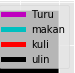
\includegraphics[width=4cm]{figures/6/1174009/legenda.png}
\caption{legenda}
\label{dwiyul}
\end{figure}

Untuk menambah label pada garis sumbu pada grafik dapat menggunakan syntax fungsi xlabel dan fungsi ylabel pada MATLAB. Kedua label ditulis setelah syntax deklarasi plot.
\lstinputlisting[firstline=47, lastline=47]{src/6/1174009/chapter6.py}
\begin{figure}[H]
\centering
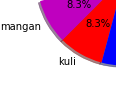
\includegraphics[width=4cm]{figures/6/1174009/label.png}
\caption{label}
\label{dwiyul}
\end{figure}


\subsubsection{soal 5}
Ketika fungsi plot dieksekusi, grafik akan ditampilkan dalam figure yang sedang aktif. Untuk beberapa kasus, perlu menampilkan plot grafik dalam figure (multiple figure) yang berbeda ataupun menampilkan lebih dari satu plot dalam satu figure. Hal ini dapat dilakukan dengan menggabungkan plot grafik dalam satu figure.
\lstinputlisting[firstline=80, lastline=80]{src/6/1174009/chapter6.py}
\begin{figure}[H]
\centering
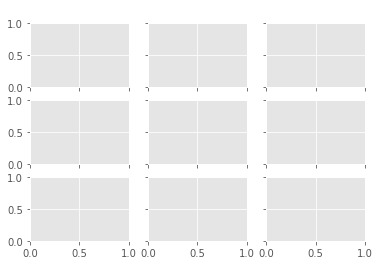
\includegraphics[width=7cm]{figures/6/1174009/multipel.png}
\caption{Histogram}
\label{dwiyul}
\end{figure}


\subsubsection{soal 6}
Kode warna yang digunakan dalam python adalah sebagai berikut:
R adalah warna Merah
G adalah warna Hijau
B adalah warna Biru
M adalah warna Ungu
Y adalah warna Kuning
C adalah warna Biru Muda
K adalah warna Hitam

\subsubsection{soal 7}
pada fungsi histogram titik koordinat tidak boleh sama karena dalam diagram ini digunakan untuk mendata selisih dari hasil rentang nilai tertentu.

\begin{figure}[H]
\centering
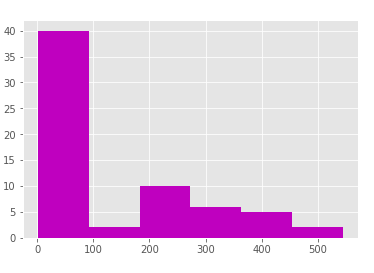
\includegraphics[width=7cm]{figures/6/1174009/1c.png}
\caption{Histogram}
\label{dwiyul}
\end{figure}


\subsubsection{soal 8}
\begin{itemize}
\item labels digunakan untuk memberi label/penjelasan dari bagian pie chart yang kita buat.
\item colors digunakan untuk mewarnai pie chart diagram yang telah dibuat, membuat warna yang berbeda antar bagian.
\item startangle digunakan untuk membuat diagram/chart mem-flip atau berbalik arah.
\item explode digunakan untuk menonjolkan salah satu bagian dari pie chart.
\item shadows digunakan untuk memberi bayangan pada pie chart yang kita buat.
\item autopct digunakan untuk memberi persen dari bagian-bagian pie chart yang kita buat.
\end{itemize}

\subsection{Bebas Plagiarisme}
\begin{figure}[H]
\centering
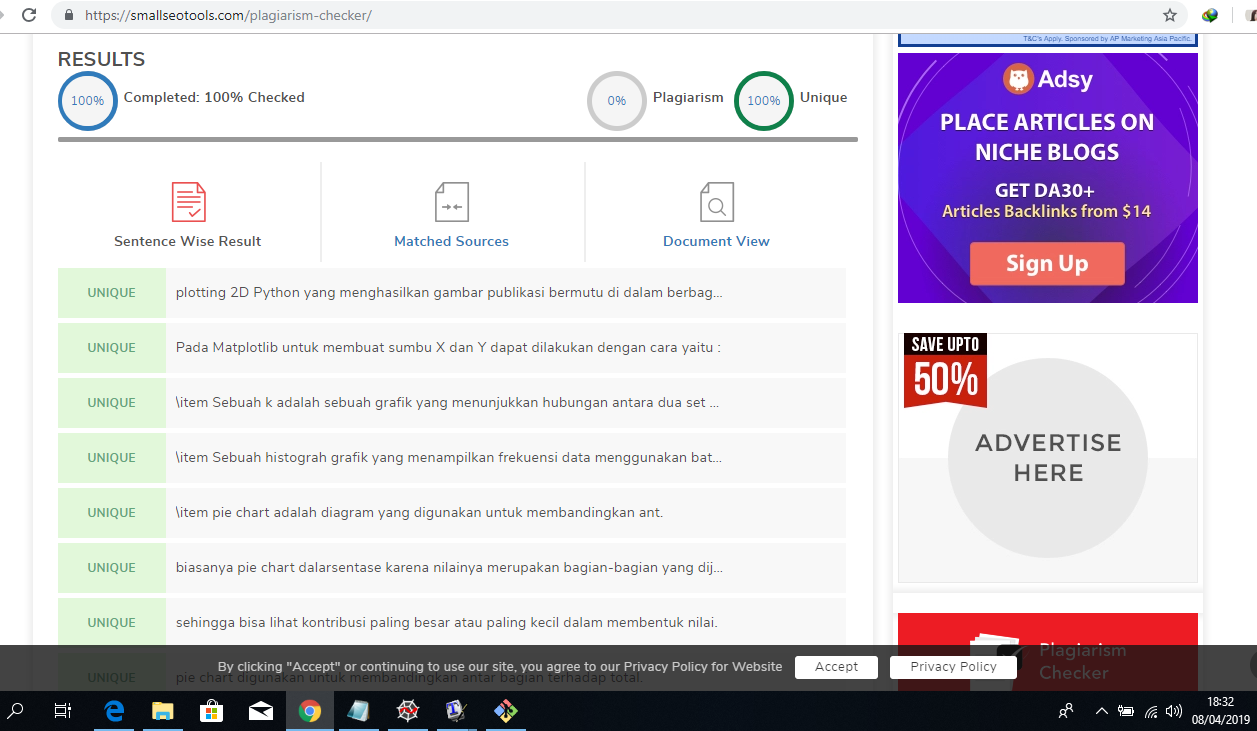
\includegraphics[width=7cm]{figures/6/1174009/plagiaris.png}
\caption{Screenshoot bebas plagiarisme mantap}
\label{dwiyul}
\end{figure}




